\documentclass[12pt]{article}

\usepackage{enumerate}
\usepackage{xcolor}
\usepackage[utf8]{inputenc}
\usepackage[greek, english]{babel}
\usepackage{alphabeta}
\usepackage{libertine}
\usepackage{graphicx}
\usepackage{biblatex}
\usepackage{wrapfig}

\title{Επαλήθευση, Επικύρωση και Συντήρηση Λογισμικού \\\large Ερευνητική Εργασία}
\author{Τσίρμπας Δημήτριος 3190205, Μανδελιάς Αλέξιος 3190106}

\pagenumbering{arabic}

\newcommand{\quotebox}[1]{\begin{center}\fcolorbox{white}{blue!15!gray!15}{\begin{minipage}{0.9\linewidth}\vspace{10pt}\center\begin{minipage}{0.8\linewidth}{\space\Huge``}{#1}{\hspace{1.5em}\break\null\Huge\hfill''}\end{minipage}\smallbreak\end{minipage}}\end{center}}

\graphicspath{ {./images/} }

\addbibresource{refs.bib}

\begin{document}

\maketitle

\section{Εισαγωγή}


Η επαλήθευση και η επικύρωση του λογισμικού ήταν ανέκαθεν μια από τις πιο σημαντικές πτυχές της ανάπτυξης λογισμικού. Η σημαντικότητα της μάλιστα έχει μόνο μεγεθυνθεί τις τελευταίες δεκαετίες, όσο η ανάπτυξη λογισμικού έχει εξελιχθεί ως πεδίο και όσο το μέγεθος και η πολυπλοκότητα των προγραμμάτων έχουν αυξηθεί. Αυτήν την στιγμή εκτιμάται ότι πάνω από 50\% του χρόνου ανάπτυξης λογισμικού καταναλώνεται στη φάση δοκιμής (testing).


\par Η επικράτηση των αντικειμενοστραφών γλωσσών προγραμματισμού έχει αλλάξει, πέρα από τον τρόπο της σχεδίασης και ανάπτυξης του λογισμικού, ριζικά και τον τρόπο εκτέλεσης της επαλήθευσης. Οι αλλαγές αυτές αφορούν όχι μόνο το πώς εκτελούνται οι μεμονωμένες δοκιμές αλλά και την ίδια την θέση της φάσης της δοκιμής στην συνολική ανάπτυξη του λογισμικού. Αντί για τις παραδοσιακές τεχνικές της ανάπτυξης του καταρράχτη (waterfall) όπου οι δοκιμές γίνονται στο τέλος κάθε σταδίου ανάπτυξης, το λογισμικό αναπτύσ\-σεται με μεθόδους συνεχούς ανάπτυξης όπως το prototyping οι οποίες απαιτούν επαναλαμβανόμενες δοκιμές για κάθε κομμάτι του λογισμικού.

\par Αυτό το γεγονός σημαίνει ότι οι παραδοσιακές τεχνικές επαλήθευσης δεν εξυπηρετούν πια τους προγραμματιστές. Οι αντικειμενοστραφείς γλώσσες, περιέχοντας έννοιες όπως απόκρυψη δεδομένων, κληρονομικότητα και κατάστασης για κάθε αντικείμενο, δεν μπορούν να εξυπηρετηθούν από την κλασσική 
αντιμετώπιση των ελέγχων ως ζευγάρια εισόδου-εξόδου ελεγμένα με έναν διαδικαστικό τρόπο. 

\par Σε αυτήν την αναφορά εξερευνούμε τις δυσκολίες που επιφέρει η χρήση του αντικειμενοστραφούς μοντέλου στην διαδικασία της επαλήθευσης, τις διαφορές της αντικειμενοστραφούς επαλήθευσης από την παραδοσιακή - διαδικαστική, θα αναλύσουμε τρόπους συμφιλίωσης αυτών των διαφορών καθώς και τεχνικές και εργαλεία που χρησιμοποιούνται για την αυτοματοποίηση και υποβοήθηση της διαδικασίας αυτής. 

\section{Διαδικαστικό vs Αντικειμενοστραφές μοντέλο επαλήθευσης}

Οι κύριες διαφορές μεταξύ των μεθόδων επαλήθευσης των δύο μοντέλων ανάπτυξης μπορούν να περιληφθούν στην εικόνα \ref{fig:hayes_table} (\textcite{hayes} as cited by \textcite{gordon}).

\begin{figure}
\label{fig:hayes_table}
\caption{Τα πιο σχετικά αξιώματα του Hayes}
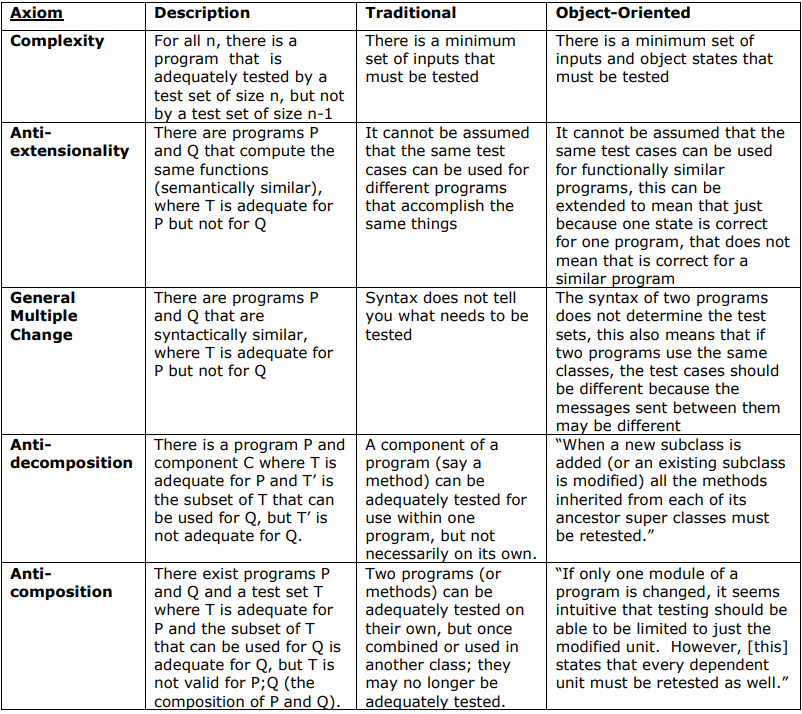
\includegraphics[width=\textwidth,height=\textheight,keepaspectratio]{hayes_table.PNG}
\end{figure}

\par Ο πίνακας αυτός αναφέρεται σε 5 από τα 11 αξιώματα του Haeys, καθώς στα υπόλοιπα είναι όμοια μεταξύ των μοντέλων ανάπτυξης σύμφωνα με τον συγγραφέα. Μπορούμε να εκτιμήσουμε λοιπόν ότι οι μισές αρχές στις οποίες βασίζονται οι έλεγχοι στο διαδικαστικό μοντέλο δεν ισχύουν στο αντικειμενοστραφές.

\par Παρακάτω περιγράφουμε αναλυτικά τις διαφορές αυτές, καθώς και τις δυσκολίες τις οποίες αυτές επιφέρουν.

\subsection{Κατάσταση}

Στο διαδικαστικό μοντέλο ένας έλεγχος μπορεί να θεωρηθεί ως ένα διατεταγμένο σύνολο ζευγών εισόδου-εξόδου. Αυτή η αναπαράσταση ισχύει επειδή το αποτέλεσμα μιας κλήσης στο μοντέλο αυτό εξαρτάται μόνο και μόνο από την είσοδο που της δίνεται.

\par Στο αντικειμενοστραφές μοντέλο κάθε αντικείμενο έχει κατά κανόνα μια εσωτερική κατάσταση. Οι πράξεις και λειτουργίες που καλούνται στο αντικείμενο αυτό όχι μόνο παράγουν εξόδους αλλά αλλάζουν και την κατάσταση αυτή (έχουν δηλαδή παρενέργειες – side effects).

\par Είναι προφανές λοιπόν πως στο αντικειμενοστραφές μοντέλο η παραπάνω αναπαράσταση δεν ισχύει, αφού το αποτέλεσμα μιας κλήσης καθορίζεται από την κατάσταση του αντικειμένου στο οποίο καλείται, η οποία μπορεί να αλλάξει από την ίδια την κλήση αλλά και από άλλες ανεξάρτητες κλήσεις. Μια επιπλέον δυσκολία είναι ότι η αλλαγή της κατάστασης δεν είναι πολλές φορές προφανής από τις εξόδους του προγράμματος.

\par Για να ανταπεξέλθουν οι έλεγχοι σε αυτές τις καινούριες απαιτήσεις, απαιτείται να συμπεριλαμβάνεται τόσο η αλλαγή της εσωτερικής κατάστασης των αντικειμένων όσο και η διαφορετική σειρά κλήσεων στις μεθόδους του αντικειμένου.

\par Πιο συγκεκριμένα σύμφωνα με τους \textcite{gordon}, για έναν ορθό και ανεπτυγμένο έλεγχο απαιτείται:

\begin{itemize}
\item Μια λίστα από μηνύματα και πράξεις που \textit{μπορεί} να εκτελεστούν από αυτόν.
\item Μια λίστα από exceptions που μπορεί ή πρέπει να πεταχτούν.
\item Ένα σταθερό περιβάλλον εκτέλεσης.
\item Όλες οι συμπληρωματικές πληροφορίες που είναι απαραίτητες στον έλεγχο.
\end{itemize}

\subsection{Πολυμορφισμός}

\par Ο πολυμορφισμός εισάγει το πρόβλημα ότι δεν υπάρχουν σταθερές υποθέσεις κατά τη διάρκεια της μεταγλώττισης. Επειδή είναι μια δυναμική λειτουργεία, δεν υπάρχει τρόπος να μαντέψουμε στον έλεγχο \textit{ποιος} κώδικας θα εκτελεστεί.

\par Οι κλάσεις στο αντικειμενοστραφές μοντέλο είναι κατά κανόνα άπειρα επεκτάσιμες και κάθε επέκταση της κλάσης μπορεί να επεκτείνει και να επαναπροσδιορίσει τις λειτουργίες κάθε κλάσης πάνω από αυτήν στην ιεραρχία. Για κάθε έλεγχο λοιπόν θα αναγκαζόμασταν να ελέγξουμε όλες τις πιθανές υποκλάσεις του κάθε αντικειμένου, πράγμα αδύνατο αφού σε οποιαδήποτε στιγμή μπορούμε να προσθέσουμε μια καινούρια υποκλάση της κλάσης του.

\par Ένα καλό παράδειγμα του προβλήματος δίνεται από τους \textcite{chandra}:

\quotebox{
Ως παράδειγμα, έστω μια μέθοδος που χρησιμοποιείται για τη σχεδίαση γραφικών. Αν περάσετε τρεις διαστάσεις, η μέθοδος draw δημιουργεί ένα τρίγωνο, αν τέσσερις ένα ορθογώνιο, πέντε πεντάγωνα κ.ο.κ. Στην περίπτωση αυτή υπάρχουν τρεις διαφορετικές μέθοδοι με το ίδιο όνομα, αλλά δέχονται διαφορετικά ποσά μεταβλητών στην κλήση της μεθόδου. Γενικά, η επιλογή της παραλλαγής καθορίζεται κατά την εκτέλεση (δυναµική δέσµευση) από τον µεταγλωττιστή µε βάση, για παράδειγµα, τον τύπο ή τον αριθµό των ορυγµάτων που παραδίδονται:

\begin{itemize}
\item Χρειαζόµαστε µόνο µία παραλλαγή;
\item Ελέγχουμε όλες τις παραλλαγές;
\item Αν όλες, χρειάζεται να τις δοκιμάσουμε όλες σε όλα τα επίπεδα;
\end{itemize}

\par Δεν υπάρχει μια συγκεκριμένη απάντηση για αυτά τα ερωτήματα. Οι απαντήσεις σε αυτά τα ερωτήματα εξαρτώνται από τους ελεγκτές, τις εταιρικές πολιτικές κ.λπ. Σε έναν τέλειο κόσμο θα δοκιμάζαμε τα πάντα. Ωστόσο, στην πραγματικότητα είναι γενικά αδύνατο να δοκιμάσουμε τα πάντα σε έργα μεγάλης κλίμακας. Οι ίδιες περιπτώσεις δοκιμών (Driver και Stubs) θα μπορούσαν να χρησιμοποιηθούν για τη δοκιμή κάθε παραλλαγής σε επίπεδο Μονάδας (επαναχρησιμοποίηση δοκιμών). Επίσης, λόγω της επαναχρησιμοποίησης του λογισμικού, μπορεί να μην είναι απαραίτητο να δοκιμαστούν όλες οι παραλλαγές σε επίπεδο Συνένωσης εάν όλες έχουν δοκιμαστεί πλήρως σε επίπεδο Μονάδας. Το αν κάθε παραλλαγή θα δοκιμαστεί σε επίπεδο συστήματος εξαρτάται από τον καθορισμό των απαιτήσεων.
}

\par Οι συγγραφείς εδώ αναφέρονται και στην λειτουργεία της δυναμικής δέσμευσης (dynamic binding). Για παράδειγμα η C++ χρησιμοποιεί κυρίως στατικό binding, το οποίο γίνεται κατά τη διάρκεια της μεταγλώττισης, για τον πολυμορφισμό, ενώ η Java κυρίως δυναμικό, μέσω του JVM (Java Virtual Machine). Στην περίπτωση της δεύτερης, επειδή το πρόγραμμα ξέρει μόνο κατά τη διάρκεια της εκτέλεσης τι τύποι παραμέτρων, επιστροφής  και άλλων δεδομένων θα χρησιμοποιηθούν, τα παραπάνω προβλήματα διογκώνονται.

\par Οι συγγραφείς τέλος συμβουλεύουν το πρόβλημα του πολυμορφισμού να μετακινηθεί όσο γίνεται στο επίπεδο ελέγχου Συστήματος και Συνένωσης αντί για το επίπεδο μονάδας.

\par Στο \textcite{chandra} μια λύση που προτείνεται είναι να οριστεί ένα συμβόλαιο ιεραρχικότητας («hierarchy specification») κατά το οποίο όλες οι υποκλάσεις συμφωνούν σε μια κοινή, ελάχιστη λειτουργικότητα. Άλλες λύσεις θα αναλυθούν αργότερα στο έγγραφο.

\subsection{Κληρονομικότητα}

Στο παραπάνω εδάφιο έγινε μια σύντομη αναφορά στο πρόβλημα του επαναπροσδιορισμού μεθόδων της υπερκλάσης. Το πρόβλημα αυτό δεν περιορίζεται μόνο στο άπειρο πλήθος των πιθανών αντικειμένων που απαντάνε μια κλήση αλλά επεκτείνεται και στο πεδίο της ίδιας της υπερκλάσης.

\par Έστω ότι έχουμε μια πλήρως ελεγμένη κλάση Α και μια υποκλάση της Β που επαναπροσδιορίζει μόνο ένα υποσύνολο των μεθόδων της Α. Θα ήταν φυσικό να υποθέσουμε ότι χρειάζεται να υλοποιήσουμε μόνο τις μεθόδους αυτές. Σύμφωνα με τους \textcite{perry} as cited by \textcite{barbey}, αυτή η υπόθεση δεν ισχύει εφόσον οι αλλαγμένες μέθοδοι ενδέχεται να χρησιμοποιούνται από κληρονομημένες, αλλάζοντας τη συμπεριφορά των δεύτερων ή να αλλάζουν την εσωτερική κατάσταση των αντικειμένων. Ένα ακόμα πρόβλημα που δημιουργεί η κληρονομικότητα είναι η παραβίαση της ενθυλάκωσης, καθώς μια υποκλάση έχει πρόσβαση - έμμεσα ή άμεσα – στα δεδομένα των υπερκλάσεών της. 

\par Αναγκαζόμαστε λοιπόν είτε να ξανά-επαληθεύσουμε όλες τις ιδιότητες της καινούριας κλάσης εκ νέου είτε να ανακαλύψουμε το ελάχιστο σύνολο από τις ιδιότητες οι οποίες είναι διαφορετικές από την κλάση-γονέα. Αλγόριθμοι και τεχνικές για την εύρεση αυτού του συνόλου δίνονται αργότερα στο έγγραφο.

\par Περιέργως, η πολλαπλή κληρονομικότητα δεν δημιουργεί προβλήματα στην διαδικασία της επαλήθευσης, τουλάχιστον όσον αφορά μοντέρνες αντικειμενοστραφείς γλώσσες (\textcite{barbey}, page 11).

\subsection{Ενθυλάκωση}

Η ενθυλάκωση (encapsulation / data hiding) είναι μια θεμελιώδης ιδιότητα του αντικειμενοστραφούς προγραμματισμού, κατά την οποία τα εσωτερικά δεδομένα ενός αντικειμένου μπορούν να αλλάξουν και να προσπελαστούν μόνο μέσω μιας διεπαφής. Εφόσον, όπως εξηγήθηκε παραπάνω, ο έλεγχος της εσωτερικής κατάστασης του αντικειμένου είναι απαραίτητος για τον έλεγχο κλάσεων, ο περιορισμός της ορατότητας δεν μας επιτρέπει να αξιολογήσουμε ορθά την κατάσταση αυτή. 

\par Οι διαισθητικές λύσεις απαιτούν  είτε να παραβούμε την ενθυλάκωση την ίδια, είτε να παράξουμε κλάσεις που μας παρέχουν μεθόδους πρόσβασης. Η πρώτη λύση παραβαίνει την λειτουργικότητα της κλάσης ενώ η δεύτερη ενδέχεται να μην λύσει το πρόβλημα, σε περιπτώσεις όπου η υποκλάση δεν έχει πρόσβαση στα εσωτερικά δεδομένα της εξεταζόμενης κλάσης.

\subsection{Μη-κατασκευάσιμες Κλάσεις}

Εφόσον στιγμιότυπα αυτών των κλάσεων δεν μπορούν να δημιουργηθούν, είναι πρακτικά αδύνατο να επαληθευτούν. Ο προγραμματιστής θα πρέπει να αναπτύξει ένα σύνολο ελέγχων το οποίο θα παρέχει προσεγγιστικά κάλυψη των κλάσεων αυτών. Δεν υπάρχει έτοιμη έρευνα στο πεδίο αυτό.\newline

\par Τέλος περιλαμβάνουμε έναν πίνακα (Πίνακας \ref{fig:panos}) από τους (\textcite{kung}) στον οποίο περιλαμβάνονται οι κύριες γενικές αλλαγές στους ελέγχους, που επιφέρουν αλλαγές στον κώδικα.

\begin{figure}
\label{fig:panos}
\caption{Πιθανές αλλαγές στον κώδικα των ελέγχων}
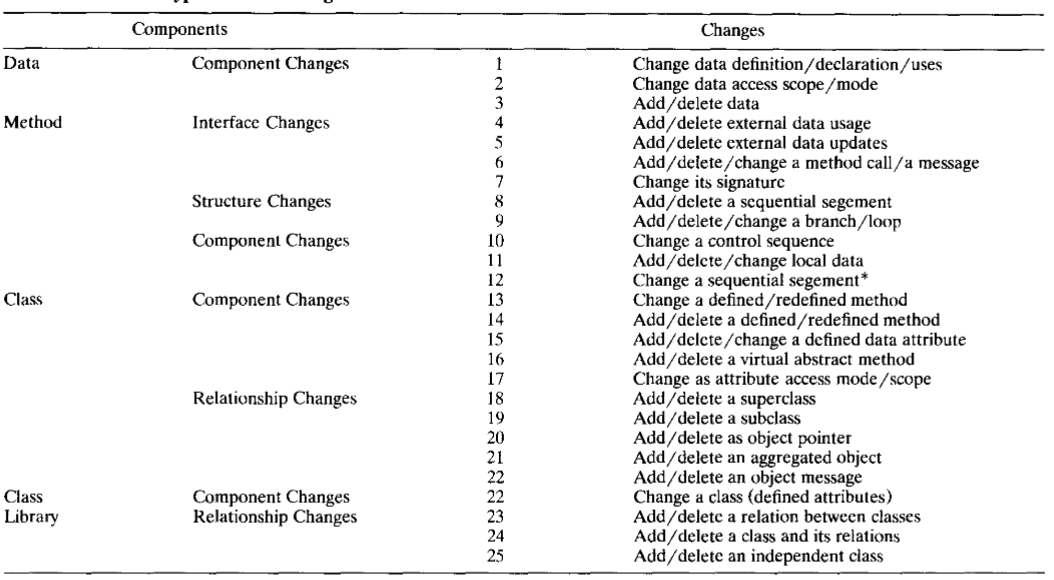
\includegraphics[width=\textwidth,height=\textheight,keepaspectratio]{code_changes_table.PNG}
\end{figure}

\section{Λύσεις}

\subsection{Έλεγχος Μονάδων}
Κατά τον Έλεγχο Μονάδων συγγράφονται περιπτώσεις ελέγχου οι οποίες καλύπτουν κατά το δυνατόν περισσότερες καταστάσεις των αντικειμένων του λογισμικού σε μια προσπάθεια εύρεσης λαθών. Όσο η πολυπλοκότητα του λογισμικού αυξάνεται, ο εξαντλητικός έλεγχος όλων των μονοπατιών εκτέλεσης και όλων των συμπεριφορών των αντικειμένων του συστήματος καθίσταται πρακτικά αδύνατος. Αυτό δυσχεραίνεται από το γεγονός ότι ο αριθμός των πιθανών καταστάσεων ενός μόνο αντικειμένου του λογισμικού είναι απαγορευτικά μεγάλος για να ελεγχθεί με το χέρι και τα εργαλεία αυτόματης κατασκευής περιπτώσεων ελέγχου κατασκευάζουν ένα επίσης απαγορευτικά μεγάλο δέντρο πιθανών καταστάσεων. Ακόμη, ο παραδοσιακός τρόπος ελέγχου με hard-coded δεδομένα αισθητά περιορίζει το πλήθος διαφορετικών μονοπατιών εκτέλεσης που όντως ελέγχονται με αποτέλεσμα μια οριστική απάντηση για το αν υπάρχουν ακόμη σφάλματα να είναι ακόμη πιο δύσκολο να δοθεί.

\subsubsection{YAQC4J}

Ο ακρογωνιαίος λίθος του εργαλείου αυτού είναι η τυχαιοποιημένη παραγωγή δεδομένων, η οποία πρωτοεμφανίστηκε στον συναρτησιακό προγραμματισμό, και συγκεκριμένα με το εργαλείο QuickCheck. Οι βασικές αρχές που διέπουν τη λειτουργεία του QuickCheck αναπροσαρμόστηκαν και επεκτάθηκαν για το αντικειμενοστραφές μοντέλο προγραμματισμού και υλοποιούνται στο εργαλείο YAQC4J το οποίο μπορεί να χρησιμοποιηθεί συμπληρωματικά με τις υπάρχουσες μεθόδους ελέγχου την αποτελεσματικότητα των οποίων επαυξάνει \cite{andres}.

\paragraph{Κεντρική Ιδέα}

Ως απάντηση στη διαρκώς αυξανόμενη πολυπλοκότητα του λογισμικού, η οποία παραπέμπει σε έναν απαγορευτικά μεγάλο αριθμό εισόδων και εξόδων που πρέπει να ελεγχθούν, το εργαλείο αυτό αυτοματοποιεί την παραγωγή των δοκιμαστικών δεδομένων επιτρέποντας στον προγραμματιστή να εκτελέσει την ίδια περίπτωση ελέγχου με έναν πολύ μεγάλο αριθμό τυχαία κατασκευασμένων αντικειμένων. Έτσι ο προγραμματιστής, τελικά, συγγράφει προδιαγραφές ελέγχου οι οποίες ελέγχονται με τη βοήθεια των τυχαιοποιημένων αντικειμένων αντί να κατασκευάζει με το χέρι πολλά διαφορετικά αντικείμενα τα οποία παρουσιάζουν μια συγκεκριμένη συμπεριφορά το καθένα.

\begin{wrapfigure}{r}{0.45\textwidth}
\centering
    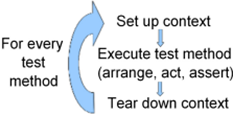
\includegraphics[width=0.35\textwidth]{conventional_testing.png}
    \caption{Διάγραμμα ελέγοχυ χρησιμοποιώντας συμβατικές μεθόδους ελέγχου λογισμικού}
    \label{fig:conventional_testing}
\end{wrapfigure}

\paragraph{Λειτουργία του Εργαλείου}

Παραδοσιακά, κάθε περίπτωση ελέγχου περιλαμβάνει την κατασκευή της αρχικής κατάστασης του αντικειμένου και ακολούθως την αποστολή των μηνυμάτων προς έλεγχο σε αυτό το αντικείμενο. Το εργαλείο YAQC4J αντικαθιστά τη διαδικασία αρχικοποίησης του αντικειμένου παρέχοντας στον προγραμματιστή τη δυνατότητα να προσδιορίσει την αρχικοποίηση αυτή παραμετρικά, με τη βοήθεια τυχαιοποιημένων αριθμών οι οποίοι προέρχονται από κάποια κατανομή την οποία μπορεί επίσης ο προγραμματιστής να ορίσει.

\par Το εργαλείο αναλαμβάνει να παραγάγει τα τυχαιοποιημένα αντικείμενα και έπειτα να εκτελέσει τις μεθόδους ελέγχου έναν μεγάλο αριθμό φορών έως ότου είτε μια εκτέλεση να αποτύχει, είτε ένας προκαθορισμένος αριθμός από εκτελέσεις να επιτύχει. Αν αποτύχει γνωρίζουμε ότι βρέθηκε κάποιο σφάλμα στο λογισμικό, αλλιώς είμαστε αρκετά βέβαιοι πως το λογισμικό δεν περιέχει σφάλματα. Η σιγουριά που εξασφαλίζεται με τη χρήση του εργαλείου είναι σαφώς μεγαλύτερη από αυτήν που έχουμε κατά τον χειροκίνητο έλεγχο καθώς το λογισμικό ελέγχεται με έναν  πολύ μεγαλύτερο αριθμό αντικειμένων σε σχέση με τις παραδοσιακές μεθόδους ελέγχου.

\begin{wrapfigure}{r}{0.45\textwidth}
\centering
    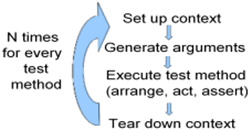
\includegraphics[width=0.35\textwidth]{testing_with_yaqc4j.png}
    \caption{Διάγραμμα ελέγχου χρησιμοποιώντας το YAQC4J}
    \label{fig:yaqc4j_testing}
\end{wrapfigure}

\subsubsection{Symstra} 

Η σημαντικότερη λειτουργία του εργαλείου αυτού έγκειται στην αυτόματη παραγωγή ελέγχων μονάδας λαμβάνοντας ως είσοδο τις μεθόδους που θα πρέπει να ελεγχθούν καθώς και το μέγιστο βάθος του δέντρου μονοπατιών εκτέλεσης. Χρησιμοποιώντας συμβολική εκτέλεση για να παρέχει στις μεθόδους συμβολικές παραμέτρους, το εργαλείο Symstra εξερευνά το δέντρο καταστάσεων του αντικειμένου και ταυτόχρονα το κλαδεύει για να πετύχει το μικρότερο δυνατό μέγεθος, εξοικονομώντας έτσι χρόνο κατά την εκτέλεση των ελέγχων.
\cite{tao}


\paragraph{Κεντρική Ιδέα}

Δεδομένων των μεθόδων προς έλεγχο, παραδοσιακά εργαλεία παραγωγής ελέγχων μονάδας ζητούν από τον χρήστη συγκεκριμένες τιμές για τα ορίσματα των μεθόδων οι οποίες συχνά δεν αρκούν για να καλύψουν όλες τις συμπεριφορές του αντικειμένου. Ακόμη ζητούν από τον χρήστη μια συνάρτηση για σύγκριση των καταστάσεων του αντικειμένου, προκειμένου να γίνει κλάδεμα του δέντρου για να μην εξεταστούν δύο ίδιοι κόμβοι, η οποία και πάλι μπορεί να είναι ελλιπής. Το εργαλείο Symstra εξάγει κατά την εκτέλεσή του τα ορίσματα που θα χρησιμοποιηθούν κατά την κλήση μεθόδων μέσω συμβολικής εκτέλεσης η οποία περιλαμβάνει τον περιορισμό που υπάρχει ως κάποιο σημείο στο δέντρο εξερεύνησης καταστάσεων και ενημερώνεται σε κάθε διακλάδωση, καθώς και τις συμβολικές μεταβλητές.

\paragraph{Λειτουργία του Εργαλείου}

\begin{wrapfigure}{r}{0.45\textwidth}
\centering
    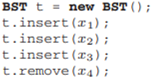
\includegraphics[width=0.35\textwidth]{bst_class.png}
    \caption{Κλάση Binary Search Tree}
    \label{fig:bst}
\end{wrapfigure}


Έστω πώς θέλουμε να ελέγξουμε το ακόλουθο αντικείμενο δέντρου δυαδικής αναζήτησης με αυτές τις 4 μεθόδους. Ορίζουμε τις συμβολικές μεταβλητές $x_1$, …, $x_4$ τις οποίες θα χρησιμοποιήσουμε κατά τη συμβολική εκτέλεση για να κατασκευάσουμε το δέντρο καταστάσεων που θα προκύψει από την εκτέλεση αυτών των εντολών. Είναι άξιο να παρατηρηθεί πως υπάρχουν καταστάσεις που έχουν διαφορετική σύνταξη (διαφορετικούς περιορισμούς) αλλά είναι σημασιολογικά ισοδύναμα καθώς μπορούμε να δώσουμε στις συμβολικές μεταβλητές ενός από αυτά συγκεκριμένες τιμές οι οποίες να ικανοποιούν τους περιορισμούς. Επομένως, δεν είναι απαραίτητο να ελέγξουμε την ισοδυναμία μεταξύ συνόλων, αλλά μόνο την «συμπερίληψη», δηλαδή ότι ένα σύνολο $s_1$ «συμπεριλαμβάνει» το $s_2$ ανν το σύνολο των συμβολικών μεταβλητών που ικανοποιεί το $s_2$ είναι υποσύνολο του συνόλου των συμβολικών μεταβλητών που ικανοποιεί το $s_1$, επομένως το εργαλείο μπορεί να αποφύγει την εξερεύνηση του $s_2$.

\begin{figure}
\label{fig:symstra_example}
\caption{"Κλαδεμένο" δέντρο εξερεύνησης χρησιμοποιώντας Symstra}
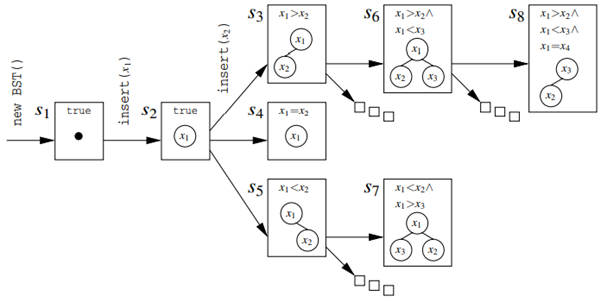
\includegraphics[width=\textwidth,height=\textheight,keepaspectratio]{symstra_example.png}
\end{figure}

\subsection{Έλεγχος Συνένωσης} 

Όσο προχωράει η ανάπτυξη του λογισμικού, δίδεται όλο και περισσότερη προσοχή στη λειτουργικότητα του λογισμικού, επομένως ο έλεγχος συνένωσης οφείλει να εξασφαλίζει τη σωστή συμπεριφορά του λογισμικού όσο συνενώνει διαφορετικές μονάδες μεταξύ τους. Οι καταστάσεις των αντικειμένων καθώς και η υπερφόρτωση μεθόδων και η δυναμική σύνδεση αντικειμένων με τις αναφορές τους καθιστούν τον έλεγχο διεπαφών δύσκολο, καθώς σε κάθε εκτέλεση και η εσωτερική κατάσταση των αντικειμένων αλλάζει, αλλά και σε κάθε κλήση μεθόδου αντιστοιχούν πιθανόν πολλές υλοποιήσεις.
Προβλήματα που πρέπει να αντιμετωπιστούν κατά τον έλεγχο συνένωσης είναι τα εξής: 1) θέλουμε να έχουμε τον σκελετό του συστήματος το νωρίτερο δυνατό, 2) κατά τη συνένωση προσέχουμε έτσι ώστε οι διεπαφές των μονάδων ενώνονται και αλληλοεπιδρούν σωστά και 3) οι μονάδες επικοινωνούν αρκούντως ικανοποιητικά έτσι ώστε να μπορεί να διεξαχθεί έλεγχος συστήματος.
\cite{bashir}

\paragraph{Προσέγγιση}

Για τον Έλεγχο Συνένωσης πρέπει να απαντήσουμε στα ακόλουθα τρία ερωτήματα:

\begin{enumerate}
  \item Πόσα αντικείμενα πρέπει να φτιάξουμε προτού αρχίσουμε τους ελέγχους;
  \item Με ποια σειρά πρέπει να συνενώσουμε τις διαφορετικές μονάδες;
  \item Χρειάζεται πάνω από ένας σκελετός για την συνένωση;
\end{enumerate}

\par Η προτεινόμενη μέθοδος που απαντάει στις 3 αυτές ερωτήσεις είναι η ακόλουθη και χρησιμοποιεί μια «εικονική μηχανή συνένωσης» που είναι υπεύθυνη να συνενώσει τα μεμονωμένα κομμάτια ενός συστήματος. Η μηχανή έχει ως είσοδο μια λίστα με τα use cases του λογισμικού καθώς και μια λίστα με τα αντικείμενα που θα χρησιμοποιηθούν. Προσπαθεί να εκτελέσει με τη σειρά κάθε use case και κάθε φορά που απαιτείται κάποιο καινούριο αντικείμενο, επιλέγεται κάποιο από τη λίστα, το οποίο ακολούθως ελέγχεται σε συνδυασμό με τα υπόλοιπα που έχουν προηγουμένως επιλεγεί για σωστή λειτουργικότητα αλλά και συνένωση.

\par Αυτή η μηχανή απαντάει στις τρεις αυτές ερωτήσεις καθώς κατασκευάζει αντικείμενα όταν αυτά χρειαστούν, οι διαφορετικές μονάδες συνενώνονται σύμφωνα με τη σειρά που καθορίζεται από το λογισμικό και παρέχει έναν σκελετό για τη συνένωση.

\subsection{Διαφορικός Έλεγχος} 

Μια από τις μεγαλύτερες δυσκολίες κατά τον έλεγχο είναι η αξιολόγηση του αποτελέσματος του ελέγχου. Τα σύγχρονα συστήματα λογισμικού είναι τόσο περίπλοκα που αποτελεί συχνά πρόκληση ο εκ των προτέρων προσδιορισμός του αναμενόμενου αποτελέσματος, πόσο μάλλον για τους τυχαιοποιημένους ελέγχους. Απαιτείται, λοιπόν, η χρήση ενός «μαντείου» με τη βοήθεια του οποίου να αποφανθούμε αν ένας έλεγχος είναι επιτυχής ή όχι. Τα καταστροφικά λάθη στο λογισμικό εντοπίζονται σχετικά εύκολα, όμως τα λογικά και σημασιολογικά λάθη δύσκολα ανιχνεύονται με παραδοσιακές μεθόδους.
\par Ο Διαφορικός Έλεγχος αποτελεί προσπάθεια εντοπισμού εκείνων των δυσεύρετων λογικών και σημασιολογικών σφαλμάτων στο λογισμικό δίνοντας την ίδια είσοδο σε πολλές παρόμοιες εφαρμογές και παρατηρώντας διαφοροποιήσεις στην έξοδο του λογισμικού ή στη συμπεριφορά του. Χρησιμοποιώντας σαν «μαντείο» τις διαφορετικές υλοποιήσεις εντοπίζονται αποκλίσεις στη συμπεριφορά των προγραμμάτων οι οποίες αποτελούν πιθανό σφάλμα στο λογισμικό.
\cite{william}
\cite{wiki}

\paragraph{Μη-Καθοδηγούμενη Παραγωγή Εισόδων}
Νέες είσοδοι παράγονται τυχαία, αγνοώντας τα αποτελέσματα των προηγούμενων εκτελέσεων. Μια τέτοια στρατηγική είναι μη αποδοτική καθώς οι είσοδοι επιλέγονται από ένα απαγορευτικά μεγάλο σύνολο πιθανών εισόδων. Η πιθανότητα εύρεσης στην τύχη εκείνων των εισόδων που θα εμφανίσουν κάποιο σφάλμα λογισμικού είναι εξαιρετικά μικρή.

\paragraph{Καθοδηγούμενη Παραγωγή Εισόδων}
Λαμβάνοντας υπόψιν πληροφορίες για τη συμπεριφορά του λογισμικού από προηγούμενες εκτελέσεις μπορούμε πιο αποδοτικά να ελέγξουμε το λογισμικό με εκείνες τις εισόδους οι οποίες είναι πιο πιθανό να αποκαλύψουν κάποιο σφάλμα του λογισμικού.

\paragraph{Εξελικτική Καθοδήγηση Ανεξάρτητη από το Πεδίο}
Χρησιμοποιώντας μετρικές λογισμικού μπορούμε να αξιολογήσουμε τις διαφοροποιήσεις μεταξύ των παρόμοιων προγραμμάτων για να αξιολογηθεί καλύτερα η ποικιλία που υπάρχει μεταξύ τους. Έτσι, εφαρμόζονται πιο αποτελεσματικά τεχνικές διαφορικού ελέγχου με μεθόδους μαύρου κουτιού που είναι ανεξάρτητες του πεδίου.

\paragraph{Συμβολική Εκτέλεση}
Αυτή η τεχνική ελέγχου άσπρου-κουτιού εκτελεί το πρόγραμμα συμβολικά, υπολογίζοντας περιορισμούς σε κάθε μονοπάτι εκτέλεσης τους οποίους έπειτα επιλύει προκειμένου να παραγάγει εισόδους που ικανοποιούν αυτούς τους περιορισμούς για κάθε μονοπάτι εκτέλεσης. Αυτή η τεχνική, αν και είναι δύσκολο να χρησιμοποιηθεί σε κλίμακα λόγω της εκθετικής πολυπλοκότητας που προκύπτει από τον αριθμό διαφορετικών μονοπατιών εκτέλεσης στα διάφορα παρόμοια προγράμματα, μπορεί να παραγάγει εισόδους για τον διαφορικό έλεγχο.

\subsection{Αρχιτεκτονική}

Η ευκολία σύνταξης σωστών ελέγχων εν μέρει εξαρτάται από τη συνοχή της κλάσης στην οποία αυτοί εφαρμόζονται (\textcite{yeresime} as cited by \textcite{gordon}). Στο διαδικαστικό μοντέλο η συνοχή (cohesion) σχετίζεται με παρόμοιες παραμέτρους και λειτουργικότητα ενώ στο αντικειμενοστραφές με το πόσο συνεκτικές είναι οι επιμέρους κλάσεις του προγράμματος. Μια κλάση θεωρείται συνεκτική αν όλες οι μέθοδοί της την ορίζουν καλά ως μια αυτοτελή μονάδα.

\par Μια κλάση με υψηλή συνοχή θα έχει μεγάλη ομοιότητα στους τύπους και τις λειτουργίες της, άρα η παραγωγή δεδομένων ελέγχου είναι εύκολη. Στην περίπτωση της χαμηλής συνοχής, η ύπαρξη πολλών ετερογενών δεδομένων και λειτουργιών σημαίνει ότι οι έλεγχοι έχουν μεγαλύτερο κόστος και είναι πιο ευάλωτοι σε σφάλματα.

\par Οι \textcite{gordon} προτείνουν μια μονάδα μέτρησης η οποία αναπαριστά την συνοχή μιας κλάσης. Παραθέτουμε τον ορισμό της:

\quotebox{
Έλλειψη συνοχής στις μεθόδους (Lack of Cohesion in Methods - LCOM) ορίζεται ως η μαθηματική διαφορά μεταξύ του αριθμού των μεθόδων των οποίων η περίπτωση μεταβλητές είναι εντελώς ανόμοιες, και του αριθμό των μεθόδων των οποίων οι μεταβλητές παραδείγματος μοιράζονται (Yeresime, et al., 2012).
\par [...]
\par Εάν η LCOM είναι υψηλή, σημαίνει ότι μια κλάση δεν είναι συνεκτική (και μπορεί να είναι υποψήφια για αναδιαμόρφωση σε δύο κλάσεις). Στο στάδιο των δοκιμών, μια κλάση θα πρέπει να έχει διαφορετικά σύνολα δοκιμών για τις διάφορες μεθόδους και όχι ένα σύνολο δοκιμών για τις ολόκληρη την κλάση. Αυτό οδηγεί σε σύγχυση και αύξηση της συνολικής πολυπλοκότητας της διαδικασίας δοκιμών.»
Σύμφωνα με τους Badri and Fadel (Badri \& Toure, 2012) η LCOM είναι μια από τις καλύτερες μονάδες για να προβλεφθεί η πολυπλοκότητα του κώδικα.
}

\par Μια δεύτερη έννοια που σχετίζεται με την ευκολία σύνταξης ελέγχων είναι η σύζευξη (coupling). Γενικά υπάρχει μια αντιστρόφως ανάλογη σχέση μεταξύ συνοχής και σύζευξης: όσο πιο πολλή συνοχή έχει μια κλάση τόσο πιο λίγη σύζευξη έχει και αντίστροφα (Khatri, et al., 2011 as cited by \textcite{gordon}). 

\par Η σύζευξη είναι μια μέτρηση που εκτιμάει τον βαθμό εξάρτησης μεταξύ κλάσεων του προγράμματος. Ενώ λοιπόν η συνοχή ασχολείται με τις σχέσεις εσωτερικά μιας κλάσης, η σύζευξη ασχολείται με τις σχέσεις \textit{μεταξύ} κλάσεων.

\par Η υψηλή σύζευξη σημαίνει ότι όλες ή οι περισσότερες μέθοδοι πρέπει να κατανοηθούν σαν ένα στενά συνδεδεμένο σύνολο, αντί για ανεξάρτητες λειτουργίες. Αυτό προφανώς επηρεάζει αρνητικά την επαλήθευση αφού οι έλεγχοι Μονάδας είναι πολύ πιο δύσκολο να γραφτούν. Η χαμηλή σύζευξη είναι ένας από τους στόχους της καλής αρχιτεκτονικής του λογισμικού, ιδιαίτερα για μεγάλα, περίπλοκα συστήματα στα οποία πρέπει να αποφεύγεται όσο το δυνατό η ανάθεση της επαλήθευσης στον έλεγχο Συστήματος και Συνένωσης.

\par Η δοκιμή των χαρακτηριστικών θα πρέπει να γίνεται σε Ελέγχους Μονάδας και κλάσης. Άλλες δοκιµές περιλαµβάνουν µεθόδους  με τιμές επιστροφής που είναι πολυμορφικές, καθώς και καθώς και πολυμορφικές παραμέτρους. Αυτό θα γίνει ευκολότερα σε συστάδες ή σε Ελέγχους Συστήματος.


\subsection{Κληρονομικότητα}

Η υλοποίηση κλάσεων είναι πιο απλή όταν γίνεται από την κορυφή της ιεραρχίας προς τα κάτω. Κατά τον ίδιο τρόπο, ο έλεγχος των κλάσεων σε μια ιεραρχία κληρονομικότητας είναι γενικά πιο απλός όταν προσεγγίζεται από την κορυφή προς τα κάτω. Εξετάζοντας πρώτα την κορυφή μιας ιεραρχίας, μπορούμε να ασχοληθούμε με την κοινή διεπαφή και τον κώδικα και στη συνέχεια με τον κώδικα του οδηγού δοκιμής για κάθε υποκλάση. Η υλοποίηση ιεραρχιών κληρονομικότητας από κάτω προς τα πάνω μπορεί να απαιτήσει σημαντική αναδιαμόρφωση του κοινού κώδικα σε μια νέα υπερκλάση. Οι πιθανότητες αντιμετώπισης διαφορετικών δομών κληρονομικότητας και η πρόσθετη δυνατότητα πιθανής αντιμετώπισης πολλαπλών μορφών κληρονομικότητας μπορεί να προσθέσει άλλο ένα επίπεδο πολυπλοκότητας στη διαδικασία δοκιμής. Τα θέματα αυτά εγείρουν μια σειρά από ερωτήματα:

\begin{itemize}
\item Ελέγχουμε πλήρως όλες τις βασικές κλάσεις και τις υποκλάσεις τους και σε ποια επίπεδα πρέπει να ελέγξουμε; 
\item Δοκιμάζουμε πλήρως όλες τις βασικές κλάσεις και μόνο τις αλλαγές ή τροποποιήσεις στις υποκλάσεις, και αν ναι σε ποια επίπεδα;
\item Με ποια σειρά ελέγχουμε την ιεραρχία, από πάνω προς τα κάτω ή από κάτω προς τα πάνω;
Για να απαντήσουμε στην 3η ερώτηση, η γενικά αποδεκτή απάντηση είναι από πάνω προς τα κάτω.
\end{itemize}

\par Οι υπόλοιπες ερωτήσεις απαντώνται κυρίως στην ενότητα της παλινδρόμησης.

\subsection{Τεχνητή Νοημοσύνη}

% TODO write some sort of intro here lmao

\par Μελετούμε τη συνεισφορά της Τεχνητής Νοημοσύνης στο έλεγχο λογισμικού εξετάζοντας πώς έχει χρησιμοποιηθεί στα διαφορετικά τμήματα του κύκλου ζωής ελέγχου λογισμικού.

\subsubsection{Επίδραση της Τεχνητής Νοημοσύνης στον Έλεγχο Λογισμικού} 


\paragraph{Προδιαγραφή των Ελέγχων}
Στην αρχή του κύκλου ζωής ελέγχου λογισμικού συγγράφονται περιπτώσεις ελέγχου σύμφωνα με τις απαιτήσεις του λογισμικού. Οι περιπτώσεις ελέγχου οργανώνονται σε ένα έγγραφο προδιαγραφών προκειμένου να εξασφαλιστεί ότι όλες οι απαιτήσεις έχουν ελεγχθεί.
\par Σε αυτήν τη διαδικασία μπορούν να χρησιμοποιηθούν Info-Fuzzy Networks (IFN) για την εκμαίευση λειτουργικών απαιτήσεων από τα δεδομένα εκτέλεσης με σκοπό την ανάκτηση ελλειπόντων ή ατελών προδιαγραφών, τον προσδιορισμό ενός ελαχίστου συνόλου ελέγχων και την αξιολόγηση της ορθότητας των εξόδων ενός λογισμικού.\cite{zubair}

\paragraph{Ξεσκαρτάρισμα Περιπτώσεων Ελέγχου}
Είναι η διαδικασία κατά την οποία επιλέγονται για εκτέλεση μόνο οι πιο αποδοτικές περιπτώσεις ελέγχου με αποτέλεσμα τη μείωση του συνολικού κόστους του ελέγχου.
\par Χρησιμοποιώντας Info-Fuzzy Networks (INF) εντοπίζονται αυτόματα συσχετίσεις μεταξύ εισόδων και των αντίστοιχων εξόδων του λογισμικού. Το INF έπειτα μαθαίνει από αυτές τις συσχετίσεις προκειμένου να δημιουργήσει ένα δέντρο κατηγοριοποίησης για τις περιπτώσεις ελέγχου από το οποίο μετά επιλέγονται οι πιο σημαντικές. Έτσι μειώνεται σημαντικά ο αριθμός συνδυαστικών ελέγχων μαύρου κουτιού.

\paragraph{Παραγωγή Περιπτώσεων Ελέγχου}
Τον προσδιορισμό κριτηρίων καταλληλότητας ελέγχου ακολουθεί η παραγωγή ενός συνόλου ελέγχων που συμμορφώνεται με αυτά τα κριτήρια. Μια τέτοια διαδικασία είναι εμφανώς υπερβολικά περίπλοκη για να εκτελεστεί με το χέρι, ειδικά για πολύπλοκα συστήματα, επομένως υπάρχει μια στροφή προς στην τεχνητή νοημοσύνη σχετικά με την αυτόματη παραγωγή των περιπτώσεων ελέγχου.
\par Αρχικά χρησιμοποιήθηκαν μέθοδοι επαγωγικής μάθησης για την παραγωγή από παραδείγματα εισόδων και εξόδων εκείνων των περιπτώσεων ελέγχου οι οποίες αρκούν για τη διαφοροποίηση του λογισμικού P που ελέγχεται από κάθε άλλο λογισμικό P’ ενός συνόλου εναλλακτικών λογισμικών.
\par Για τον έλεγχο μαύρου κουτιού κατασκευάζεται ένα μοντέλο της συμπεριφοράς του λογισμικού μέσω παραδειγμάτων εισόδων-εξόδων, το οποίο χρησιμοποιείται για να δημιουργήσει νέες εισόδους.
\par Περιπτώσεις ελέγχου μπορούν να παραχθούν αναλύοντας απευθείας το Έγγραφο Προσδιορισμού Απαιτήσεων Λογισμικού χρησιμοποιώντας τεχνικές επεξεργασίας φυσικής γλώσσας (Natural Language Processing, NLP).

\paragraph{Παραγωγή Δεδομένων Ελέγχου}
Για την εκτέλεση των Περιπτώσεων Ελέγχου απαιτείται παραγωγή των δεδομένων τα οποία θα χρησιμοποιηθούν για τον έλεγχο του λογισμικού. Όσο καλύτερη είναι η ποιότητα αυτών των δεδομένων τόσο μεγαλύτερη θα είναι και η κάλυψη του κώδικα από τις περιπτώσεις ελέγχου.
\par Με τη βοήθεια γενετικών αλγορίθμων πραγματοποιείται αναζήτηση στον χώρο των εισόδων του λογισμικού για την εύρεση δεδομένων τα οποία καλύπτουν κάθε μονοπάτι εκτέλεσης.
\par Χρησιμοποιώντας βαθιά μάθηση, με τη μέθοδο «μαϊμού» γίνεται εκμάθηση των εισόδων που θα έβαζε ο ελεγκτής του λογισμικού και στατιστική συσχέτισή τους με τα συμφραζόμενα. Ακολούθως η «μαϊμού» προβλέπει νέες εισόδους με βάση τα παρατηρούμενα συμφραζόμενα σε κάθε περίπτωση.

\paragraph{Κατασκευή «Μαντείου» (Oracle) Ελέγχου}
Προκειμένου να επιτελέσει ο έλεγχος λογισμικού σωστά τη λειτουργεία του χρειάζεται ένας μηχανισμός ο οποίος να έχει τη δυνατότητα, δεδομένης μιας εισόδου στο λογισμικό, να διαχωρίσει τη σωστή και λανθάνουσα συμπεριφορά του λογισμικού. Αυτός ο μηχανισμός αποτελεί το πρόβλημα του μαντείου (oracle problem).
\par Αλγόριθμοι μηχανικής μάθησης μπορούν να χρησιμοποιηθούν για την αυτόματη κατασκευή μαντείων, ακόμα και σε περιπτώσεις όπου οι προδιαγραφές λογισμικού είναι ελλιπείς. Κάθε εκτέλεση του ελέγχου παράγει αποτελέσματα με τα οποία τροφοδοτείται ο αλγόριθμος. Το μοντέλο που προκύπτει χρησιμοποιείται ως το μαντείο.
\par Όταν υπάρχει ένα μοντέλο αναφοράς του λογισμικού, τότε μπορεί επίσης να χρησιμοποιηθεί επιβλεπόμενη μηχανική μάθηση μέσω της οποίας το μοντέλο που προκύπτει μαθαίνει να διαχωρίσει τις περιπτώσεις ελέγχου ως επιτυχείς και ανεπιτυχείς.
\par Η επιβλεπόμενη μάθηση εφαρμόζεται και σε νευρωνικά δίκτυα, όπου το μοντέλο μαθαίνει να διαχωρίζει μοτίβα εκτέλεσης για επιτυχείς και μη εκτελέσεις για ένα δοσμένο λογισμικό. Ένα μικρό υποσύνολο των ιχνών εκτέλεσης κατηγοριοποιούνται ως επιτυχείς ή μη και το μοντέλο έπειτα μαθαίνει από αυτά.

\paragraph{Ιεράρχηση Περιπτώσεων Ελέγχου}
Οι διάφορες περιπτώσεις ελέγχου μπορούν να εκτελεστούν με πολλούς διαφορετικούς τρόπους. Προσπαθούμε να βρούμε τη βέλτιστη σειρά εκτέλεσης έτσι ώστε να δοθεί προτεραιότητα σε αυτές τις περιπτώσεις ελέγχου οι οποίες είναι πιο πιθανό να αποκαλύψουν ατέλειες του λογισμικού, ή σε αυτές οι οποίες συσχετίζονται με μεγαλύτερο κίνδυνο ανάλογα με, φερ’ ειπείν, τη σοβαρότητα του αντικειμένου υπό έλεγχο ή την επίπτωση του κινδύνου εάν εμφανιστεί.
\par Ένα σύνολο υπάρχουσων τεχνικών συνενώνεται και λειτουργεί ως μηχανική μάθηση για την ιεράρχηση περιπτώσεων ελέγχου χρησιμοποιώντας πληροφορίες κάλυψης του κώδικα, ηλικία του ελέγχου, ιστορικό αποτυχιών και ομοιότητα του κειμενικού περιεχομένου, προκειμένου να κατασκευάσει ένα μοντέλο που ιεραρχεί αποτελεσματικά περιπτώσεις ελέγχου
\par Για την Κατάταξη SVM (support-vector machines, επίσης ως και support-vector networks) χρησιμοποιούνται μετά-δεδομένα μαύρου κουτιού, όπως ιστορικό περιπτώσεων ελέγχου, αλλά και οι περιγραφές των περιπτώσεων ελέγχου σε φυσική γλώσσα προκειμένου να ιεραρχηθούν οι περιπτώσεις χρήσης.

\paragraph{Εκτίμηση του Κόστους των Περιπτώσεων Ελέγχου}
Η εκτίμηση του κόστους είναι η διαδικασία κατά την οποία προβλέπεται η απαιτούμενη προσπάθεια για την ανάπτυξη του λογισμικού. Γενικά δε θα έπρεπε να υπάρχει έλλειμα στην εκτίμηση, και αυτή θα πρέπει να είναι διαθέσιμη το νωρίτερο δυνατό.
\par Μοντελοποιώντας το κόστος ως ένα τρισδιάστατο διάνυσμα του αριθμού των περιπτώσεων ελέγχου, της πολυπλοκότητας εκτέλεσης του ελέγχου και των ανθρώπων που ελέγχουν το λογισμικό, δημιουργείται μια βάση με προηγούμενα δεδομένα πάνω στην οποία εφαρμόζεται SVM για την εκτίμηση του κόστους για δεδομένα ιστορικά δεδομένα και διανύσματα που μοντελοποιούν το κόστος.
\par Η μηχανική μάθηση μπορεί να προβλέψει το μέγεθος του κώδικα ελέγχου, δηλαδή τη μετρική λογισμικού «γραμμές κώδικα ελέγχου», που αποτελεί σημαντικό δείκτη της προσπάθειας που θα καταβληθεί κατά τον έλεγχο. Χρησιμοποιώντας τεχνικές όπως γραμμική παλινδρόμηση, Κ-κοντινότεροι-γείτονες, αφελής ταξινομητής Bayes, τυχαίο δάσος και Perceptron πολλαπλών επιπέδων κατασκευάστηκε μοντέλο που με ακρίβεια προβλέπει αυτήν τη μετρική.
\par Επειδή η υποεκτίμηση του κόστους έχει σοβαρές συνέπειες στην ποιότητα του λογισμικού, τα μοντέλα που εκτιμούν το κόστος περιλαμβάνουν κάποια προκατάληψη προς την υπερεκτίμηση. Ακόμη, εντοπίζονται τα χαρακτηριστικά εκείνα που είναι πιο σημαντικά για την πρόβλεψη του κόστους ελέγχου λογισμικού, και συγκεκριμένα του χρόνου ελέγχου.


\begin{table}[]
\begin{tabular}{|p{5cm}|p{10cm}|}
\hline
\textbf{Software Testing Activity} & \textbf{AI Technique Applied}                                                                                                                                                                                                                                                                          \\ \hline
Test Case Generation               & Inductive Learning - Active Learning - Ant colony Optimization - Markov Model - AI Planner -GA - Tabu Search - NLP - Re-enforcement Learning C4.5 - Goal Based - Decision Tree - K-Nearest Neighbour - Logistic Regression - Random Forest - Multi-Layer Perceptron - K star - LSTM - Heuristic Search \\ \hline
Test Data Generation               & GA - Simulated Annealing - Hill Climbing - Generative Model - LSTM - Deep Re-enforcement Learning - Ant Colony Optimization - Heuristic Methods                                                                                                                                                        \\ \hline
Test Oracle Construction           & ANN - SVM - Decision Trees - AdaBoostM1 - Incremental Reduced Error Pruning (IREP) - Info Fuzzy Network                                                                                                                                                                                                \\ \hline
Test Case Prioritization           & K-Means - Expectation-Maximization - c4.5 - Cob Web - Reinforcement Learning - CBR - ANN - Markov Model - K-NN - Logistic Regression - SVM Rank                                                                                                                                                        \\ \hline
Test Case Specification            & IFN - C4.5                                                                                                                                                                                                                                                                                             \\ \hline
Test Case Refinement               & IFN - Classification Tree Method                                                                                                                                                                                                                                                                       \\ \hline
Test Cost Estimation               & SVM - linear regression - k-NN - Naïve Bayes - C4.5 - Random Forest - Multilayer Perceptron                                                                                                                                                                                                            \\ \hline
\end{tabular}
\caption{Τεχνικές που εφαρμόζονται ανά τύπο δραστηριότητας ελέγχου}
\end{table}


\subsubsection{Γενετικοί Αλγόριθμοι}

Όπως και στο διαδικαστικό μοντέλο, έτσι και στο αντικειμενοστραφές, ο έλεγχος περιπτώσεων δοκιμών μεγάλου μεγέθους θα μπορούσε να καταστήσει ανέφικτη την εκτέλεση όλων των πιθανών περιπτώσεων δοκιμής για την επαλήθευση του προγράμματος. Μια λύση σε αυτό το πρόβλημα είναι η τυχαία δοκιμή. Οι \textcite{ciupa} παρέχουν αποδείξεις ότι ο σχετικός αριθμός σφαλμάτων που ανιχνεύονται από τυχαίο έλεγχο με την πάροδο του χρόνου είναι προβλέψιμος και μάλιστα ότι αυτός βρίσκει σφάλματα σχετικά γρήγορα. Η πρώτη αποτυχία είναι πιθανό να προκληθεί εντός 30 δευτερολέπτων. Οι εξελικτικοί αλγόριθμοι όπως οι γενετικοί αλγόριθμοι έχουν χρησιμοποιηθεί ευρέως για διαδικαστικούς δοκιμές λογισμικού. Σε ορισμένα μέρη, προσεγγίσεις που βασίζονται σε γενετικούς αλγορίθμους έχουν προταθεί για τη δοκιμή αντικειμενοστραφούς λογισμικού.

\par Μια διαισθητική χρήση γενετικού προγραμματισμού είναι να κατασκευαστούν έλεγχοι οι οποίοι αποτελούνται από μια ακολουθία κλήσεων μεθόδων. Αυτό θα μπορούσε να υλοποιηθεί κωδικοποιώντας μεθόδους σαν αναγνωριστικά τα οποία ο αλγόριθμος θα αξιολογούσε χρησιμοποιώντας μια μέθοδο καταλληλότητας (fitness function). Παρόλα αυτά αποδείχτηκε ότι η υλοποίηση αυτή παράγει τόσο πολλές άκυρες ακολουθίες κλήσεων που ο αλγόριθμος δεν είναι αποδοτικός.

\par Στο \textcite{meziane} γίνεται αναφορά στους \textcite{wappler}), οι οποίοι χρησιμοποίησαν επίσης γενετικό προγραμματισμό, όχι για random testing, αλλά για να παραχτούν αυτόματοι έλεγχοι με την παραγωγή και εξέλιξη δέντρων τα οποία αναπαριστούν συναρτήσεις ή μεθόδους. Η ακριβής υλοποίηση δίνεται παρακάτω:

\quotebox{
Η βασική αναπαράσταση με τα περισσότερα συστήματα GP είναι ένα δέντρο αντί για μια αριθμητική λίστα. Γενικά, ένα δέντρο αναπαριστά μια συνάρτηση, όπου οι κόμβοι των φύλλων αναπαριστούν τα ορίσματα και οι μη τερματικοί κόμβοι τις συναρτήσεις. Στο πλαίσιο των δοκιμών, τα δέντρα αυτά μπορούν να αναπαραστήσουν τις εξαρτήσεις μεταξύ των κλήσεων μεθόδων, οι οποίες μπορούν στη συνέχεια να γραμμικοποιηθούν για την παραγωγή δοκιμών. Η χρήση της μετάλλαξης και της διασταύρωσης σε αυτά τα δέντρα μπορεί να οδηγήσει σε άκυρες συναρτήσεις και ακατάλληλα ορίσματα στο πλαίσιο της δοκιμής αντικειμενοστραφών προγραμμάτων. 
}

\quotebox{Ως εκ τούτου, οι Wappler και Wegener(2006), προτείνουν τη χρήση ισχυρά τυποποιημένων GP (Montana, 1995), όπου οι τύποι των κόμβων χρησιμοποιούνται για να διασφαλιστεί ότι εξελίσσονται μόνο δέντρα με κατάλληλα ορίσματα. Αυτό εξακολουθεί να αφήνει ανοιχτό το ζήτημα του τρόπου με τον οποίο λαμβάνονται αυτά τα δέντρα κατ' αρχάς. Η προσέγγιση που υιοθετούν είναι να ληφθεί πρώτα ένας γράφος εξάρτησης κλήσης μεθόδου που έχει συνδέσμους μεταξύ κόμβων κλάσης και κόμβων μεθόδου. Οι σύνδεσμοι καθορίζουν τις μεθόδους που μπορούν να χρησιμοποιηθούν για τη δημιουργία περιπτώσεων μιας κλάσης και ποιες περιπτώσεις χρειάζονται από μια συγκεκριμένη μέθοδο. Αυτός ο γράφος μπορεί στη συνέχεια να διανυθεί για τη δημιουργία δέντρων που θα παρέχουν τον αρχικό πληθυσμό. Τα απαιτούμενα ορίσματα (αντικείμενα) για τα δέντρα λαμβάνονται από μια διαδικασία δεύτερου επιπέδου που περιλαμβάνει αρχικά τη δημιουργία γραμμικών ακολουθιών κλήσης μεθόδων από τα δέντρα και στη συνέχεια χρησιμοποιεί έναν ΓΑ για την εύρεση των πιο κατάλληλων υλοποιήσεων. Μόλις επιτευχθεί αυτό, τα δέντρα βελτιστοποιούνται με τη χρήση επανασυνδυασμού και μεταλλάξεων σε σχέση με στόχους, όπως η κάλυψη της μεθόδου.}

\par Μια σημαντική βελτίωση στο έργο των Wappler and Wegener έφερε ο Ribeiro (2008), ο οποίος εκτέλεσε τον παραπάνω αλγόριθμο αγνοώντας μεθόδους που δεν είχαν καμία παρενέργεια (δηλαδή δεν μετέβαλλαν την εσωτερική κατάσταση του αντικειμένου τους). Μια δοκιμή στην κλάση Stack της Java Standard Library απέδειξε ότι αυτή η βελτίωσε μείωσε το χρόνο εκτέλεσης κατά δύο τρίτα για να αποκτηθεί πλήρης κάλυψη.

\par Οι \textcite{meziane} αναφέρουν και μια ακόμα ενδιαφέρουσα χρήση γενετικών αλγορίθμων στο πεδίο της ανάπτυξης ελέγχων:

\par Οι \textcite{briand} διερευνούν τη χρήση ΓΑ για τον προσδιορισμό της βέλτιστης σειράς για την ενσωμάτωση και τη δοκιμή κλάσεων. Ένα σημαντικό πρόβλημα κατά τον προσδιορισμό της κατάλληλης σειράς εμφανίζεται επειδή πρέπει να σπάσουν οι κύκλοι εξάρτησης των κλάσεων με αποτέλεσμα να είναι απαραίτητη η χρήση stubs. Η πολυπλοκότητα των απαιτούμενων stubs ποικίλλει, ανάλογα με το επίπεδο σύζευξης που υπάρχει μεταξύ των κλάσεων, συνεπώς διαφορετικές διατάξεις απαιτούν διαφορετικά επίπεδα προσπάθειας για τη δημιουργία των stubs. 

\par Οι \textcite{briand} εκμεταλλεύονται προηγούμενες εργασίες για τον προγραμματισμό, για παράδειγμα στη χρήση ΓΑ για το πρόβλημα του πλανόδιου πωλητή, και χρησιμοποιούν μια κωδικοποίηση των κλάσεων με μεταθέσεις μαζί με μια συνάρτηση καταλληλότητας που μετρά το βαθμό σύζευξης μεταξύ των κλάσεων. Το μέτρο καταλληλότητας ορίζεται έτσι ώστε να μειώνεται ο αριθμός των χαρακτηριστικών, οι μέθοδοι που θα χρειαζόταν να χειριστούν αν αποκοπεί μια εξάρτηση και ο αριθμός των stubs που δημιουργούνται. Επιπλέον, δεν επιτρέπουν την αποκοπή των εξαρτήσεων κληρονομικότητας και σύνθεσης, καθώς οδηγούν σε δαπανηρά stubs. Πειραματίζονται με αυτή την προσέγγιση σε μια μελέτη περίπτωσης ΑΤΜ χρησιμοποιώντας το σύστημα ΓΑ Evolver (Palisade, 1998), συγκρίνουν τα αποτελέσματα με εκείνα που προέκυψαν με τη χρήση μιας προσέγγισης βασισμένης σε γράφους και καταλήγουν στο συμπέρασμα ότι η χρήση ΓΑ μπορεί να παρέχει μια καλύτερη προσέγγιση για την παραγωγή διατάξεων ενσωμάτωσης και δοκιμής κλάσεων.

\subsubsection{Νευρωνικά δίκτυα}

Στο \textcite{chandra} γίνεται αναφορά στο έργο των \textcite{gong}. οι οποίοι πρότειναν την χρήση Event-Driven Petri Nets (EDPN) έτσι ώστε να μοντελοποιηθούν οι μεταβολές στην εσωτερική κατάσταση και στην συμπεριφορά των αντικειμένων.

\quotebox{
Τα σφάλματα ανιχνεύονται με την ανάλυση των διαφορών των σεναρίων δοκιμής στις δυναμικές συμπεριφορές των EDPN και η μέθοδος μπορεί να επιλέξει μια περίπτωση δοκιμής που ανιχνεύει σφάλματα που περιγράφονται στα μοντέλα σφαλμάτων. Οι Ghang et al. πρότειναν μια μέθοδο που χρησιμοποιεί ελέγχους σχετικής αξιοπιστίας και λειτουργίας πρόβλεψης της αξιοπιστίας των μονοπατιών για την προσαρμογή της κατανομής των δοκιμών αξιοπιστίας λογισμικού σε αντικειμενοστραφή προγραμματισμό. Στη προσέγγισή τους, η δοκιμή αξιοπιστίας λογισμικού βασίζεται στα προφίλ λειτουργίας και την πρόβλεψη της σχετικής αξιοπιστίας των μονοπατιών λειτουργίας. Για το σκοπό αυτό χρησιμοποίησαν έναν αλγόριθμο μάθησης νευρωνικού δικτύου.
}

\par Μέχρι στιγμής το έγγραφο αυτό έχει επικεντρωθεί αποκλειστικά στην επαλήθευση του λογισμικού, εφόσον είναι το θέμα το οποίο καταναλώνει τον περισσότερο χρόνο και είναι πιο άμεσα σχετικό με το αντικειμενοστραφές μοντέλο. Παρόλα αυτά η επικύρωση του λογισμικού, ο έλεγχος ότι η λειτουργικότητα του λογισμικού ανταποκρίνεται στις απαιτήσεις του πελάτη, είναι ένα εξίσου σημαντικό κομμάτι της διαδικασίας ανάπτυξης. Εδώ τα νευρωνικά δίκτυα μπορούν να μας βοηθήσουν μέσω της ανάλυσης των γραπτών σε φυσική γλώσσα απαιτήσεων του πελάτη και την μετατροπή τους σε μορφή κατάλληλη για τους σχεδιαστές και τους προγραμματιστές αποφεύγοντας ανθρώπινα λάθη στην διαδικασία αυτή.

\par Οι \textcite{feras} περιγράφουν ένα τέτοιο σύστημα:

\quotebox{
Οι περιπτώσεις χρήσης που προέκυψαν ήταν σαφείς και συνεπείς, ανεξάρτητα από το μέγεθος του κειμένου των απαιτήσεων. Τα R-Tool, NL-OOPS, CM-BUILDER είναι μερικά άλλα εργαλεία μηχανικής λογισμικού με τη βοήθεια υπολογιστή που βασίζονται σε NLP. Τα εργαλεία αυτά παράγουν διαγράμματα κλάσεων από το έγγραφο απαιτήσεων χρήστη (αν και εξακολουθεί να απαιτεί την παρέμβαση του χρήστη). 

\par Οι Michl et al. πρότειναν το NL-OOPS (Natural Language - Object-Oriented Production System) για την ανάπτυξη ενός εργαλείου που υποστηρίζει αντικειμενοστραφή ανάλυση. Τα έγγραφα απαιτήσεων αναλύονται με το LOLITA (Large-scale Object-based Linguistic Interactor, Translator and Analyzer), ένα σύστημα επεξεργασίας ΝΛ μεγάλης κλίμακας. Και τα δύο, το γνώσεις που περιέχονται στα έγγραφα όσο και αυτές που είναι ήδη αποθηκευμένες στη Βάση Γνώσης του LOLITA προτείνεται στη συνέχεια να χρησιμοποιηθούν για την παραγωγή μοντέλων απαιτήσεων. Η προσέγγιση ήταν βασισμένη στη θεώρηση ότι οι απαιτήσεις συχνά γράφονται σε αδόμητη φυσική γλώσσα και σε πολλά περιπτώσεις, είναι αδύνατο να επιβληθούν περιορισμοί πελατών στη γλώσσα που χρησιμοποιείται. 

\par Η αντικειμενοστραφής μονάδα μοντελοποίησης υλοποίησε έναν αλγόριθμο που φιλτράρει τους κόμβους οντοτήτων και συμβάντων στη γνώση του βάση δεδομένων για τον εντοπισμό κλάσεων και συσχετίσεων. Παράλληλα, οι Ninaus et al. πρότειναν μια μέθοδο για την μείωση του κινδύνου απαιτήσεων χαμηλής ποιότητας μέσω της βελτίωσης της υποστήριξης των ενδιαφερόμενων μερών σε ανάπτυξης μοντέλων RE. Οι συγγραφείς εισήγαγαν το περιβάλλον INTELLIREQ. Αυτό το περιβάλλον βασίζεται σε διαφορετικές προσεγγίσεις συστάσεων που υποστηρίζουν τα ενδιαφερόμενα μέρη στην δραστηριότητες που σχετίζονται με τις απαιτήσεις, όπως ο ορισμός, η διασφάλιση της ποιότητας, η επαναχρησιμοποίηση και ο σχεδιασμός έκδοσης.
}


\subsubsection{Δοκιμές Παλινδρόμησης}

Σύμφωνα με τους \textcite{kung}, ο έλεγχος παλινδρόμησης πρέπει να αντιμετωπίσει τέσσερα θεμελιώδη προβλήματα:

\begin{itemize}
\item Πώς να προσδιορίσουμε αυτόματα τα στοιχεία που έχουν επηρεαστεί λόγω αλλαγής ορισμένων άλλων στοιχείων.
\item Ποια στρατηγική πρέπει να χρησιμοποιηθεί για την επαναληπτική δοκιμή αυτών των επηρεασμένων στοιχείων.
\item Ποια είναι τα κριτήρια κάλυψης για τον επανέλεγχο αυτών των στοιχείων.
\item Πώς να επιλέξουμε, να επαναχρησιμοποιήσουμε και να τροποποιήσουμε τον υπάρχοντα έλεγχο (και να δημιουργηθούν νέοι).
\end{itemize} 


\par Λύσεις σε αυτά τα προβλήματα για τα παραδοσιακά προγράμματα έχουν προταθεί τις τελευταίες δύο δεκαετίες. Ωστόσο, η δοκιμή των αντικειμενοστραφών (00) προγραμμάτων έχει τύχει πολύ μικρής προσοχής, ενώ η παλινδρόμηση δεν έχει λάβει σχεδόν καθόλου. Αυτό γίνεται για τρείς κύριους λόγους σύμφωνα με τον συγγραφέα:

\par Πρώτον, οι παραδοσιακές προσεγγίσεις δεν αντιμετωπίζουν τις πολύπλοκες σχέσεις και εξαρτήσεις, όπως η κληρονομικότητα, η συνάθροιση και η συσχέτιση, που υπάρχουν μεταξύ των κλάσεων. Δεύτερον, οι περισσότερες παραδοσιακές προσεγγίσεις βασίζονται στο μοντέλο ροής ελέγχου, αλλά τα αντικείμενα των κλάσεων έχουν συμπεριφορά εξαρτώμενη από την κατάσταση που μπορεί να αλλάξει με διάφορους τρόπους- ως εκ τούτου, οι παραδοσιακές προσεγγίσεις δεν μπορούν να εφαρμοστούν στη δοκιμή κλάσεων. Τρίτον, οι παραδοσιακές προσεγγίσεις χρησιμοποιούν stubs δοκιμών για να προσομοιώσουν τις μονάδες που καλούνται, αλλά σε αντικειμενοστραφή προγράμματα αυτό είναι δύσκολο και δαπανηρό, επειδή απαιτεί την κατανόηση πολλών σχετικών κλάσεων, των συναρτήσεων-μελών τους και του τρόπου με τον οποίο καλούνται οι συναρτήσεις-μέλη.

\par Θα παρατηρήσουμε τώρα δύο προσεγγίσεις στην χρήση της παλινδρόμησης για τη λύση των προβλημάτων που παρουσιάζει η επαλήθευση αντικειμενοστραφών γλωσσών προγραμματισμού:

\par Στο \textcite{divya} χρησιμοποιείται γραμμική παλινδρόμηση σε αρχεία πηγαίου κώδικα java για να παραχθεί το ελάχιστο σύνολο ελέγχων που πρέπει να εκτελεστούν ώστε να έχει αντιμετωπιστεί η μεγάλη πλειοψηφία πιθανών σφαλμάτων.

\begin{figure}
\label{fig:regression}
\caption{Το πλάνο εκτέλεσης του προγράμματος των \textcite{divya}}
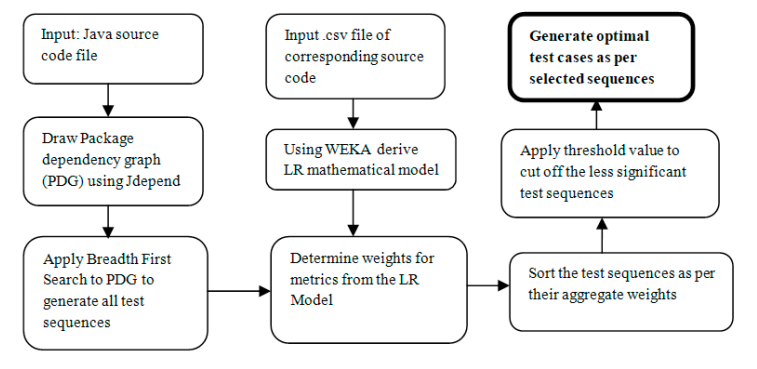
\includegraphics[width=\textwidth,height=\textheight,keepaspectratio]{regression_plan.PNG}
\end{figure}

\par Ακολουθεί μια περίληψη των βημάτων που εκτελέστηκαν έτσι ώστε να παραχθεί το παραπάνω σύνολο:

\begin{itemize}
\item Εισαγωγή του πηγαίου κώδικα Java και του αρχείου .csv: Αυτό το βήμα λαμβάνει ως είσοδο τον πηγαίο κώδικα Java απαλλαγμένος από όλα τα συντακτικά λάθη. Λαμβάνεται σύνολο δεδομένων που περιέχει τις μετρήσεις διαφόρων αντικειμενοστραφών μετρικών και τον αριθμό των σφαλμάτων που υπάρχουν στο κώδικα. Μετά από όλη την απαιτούμενη προεπεξεργασία το αρχείο .csv δόθηκε στο λογισμικό WEKA για την εκτέλεση περαιτέρω βημάτων.

\item Σχεδίαση PDG (Package Depedency Graph) και εξαγωγή μαθηματικού μοντέλου: Προκειμένου να σχεδιαστεί το PDG από το δεδομένο αρχείο .jar, χρησιμοποιήθηκε το Jdepend. Εφαρμόζεται το μοντέλο γραμμικής παλινδρόμησης (LR) μεταξύ των μετρικών και των σφαλμάτων που υπάρχουν στο ενότητες λογισμικού προέκυψε μέσω της εφαρμογής του WEKA.

\item Προκειμένου να γνωρίζουμε όλες τις πιθανές ακολουθίες ελέγχων για το PDG γράφημα, εφαρμόζεται η τεχνική BFS (Breadth First Search).

\item Καθορισμός των βαρών των μετρικών: από το μοντέλο LR που προέκυψε στο βήμα 2, τα βάρη των μετρικών είναι με βάση τους αντίστοιχους συντελεστές.

\item Ταξινόμηση των ακολουθιών δοκιμής: Η ταξινόμηση των ακολουθιών δοκιμών γίνεται με βάση τα αθροιστικά τους βάρη. 

\item Μετά την εφαρμογή ενός κατωφλίου στα αθροιστικά βάρη, μπορούν να επιλεγούν οι κορυφαίες n ακολουθίες δοκιμών. Κατώφλι για την παρούσα μελέτη είναι το 50\% του βάρους.

\item Οι βέλτιστες περιπτώσεις δοκιμών μπορούν να παραχθούν από τις επιλεγμένες n ακολουθίες δοκιμών.

\end{itemize}
 
\begin{figure}
\label{fig:pdg_graph}
\caption{Ο γράφος PDG για τη βιβλιοθήκη apache camel της Java}
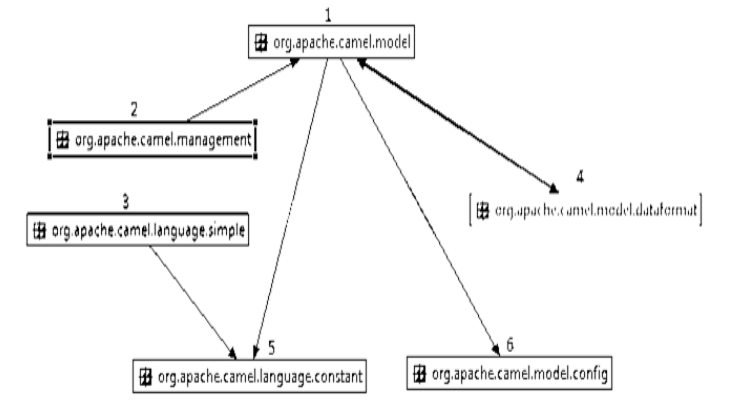
\includegraphics[width=\textwidth,height=\textheight,keepaspectratio]{pdg_graph.PNG}
\end{figure}

\par Ο αλγόριθμος εξετάζει πολλές μονάδες αξιολόγησης του λογισμικού, μερικές στις οποίες έχουμε ήδη αναφερθεί (σαν το LCOM) και αξιολογεί πόσο «συνεισφέρει» κάθε μονάδα στην πιθανότητα κάποιου bug. Το λογισμικό WAKA παράγει μια πρωτοβάθμια εξίσωση στην οποία κάθε μονάδα είναι μια παράμετρος. Αντικαθιστώντας κάθε παράμετρο με την μονάδα του κάθε λογισμικού παράγεται ένας αριθμός που αξιολογεί την καταλληλότητα ενός ελέγχου να βρίσκει σφάλματα. 

\par Τέλος, ταξινομούμε κάθε ακολουθία από ελέγχους με βάση την παραπάνω τιμή και μπορούμε να φτιάξουμε έναν πίνακα (Πίνακας \ref{fig:test_table}) με τους πιο αποτελεσματικούς ελέγχους. Στο παρακάτω παράδειγμα αυτές θα ήταν οι TS3, TS4, TS5, TS6, TS7, TS10.

\begin{figure}
\label{fig:test_table}
\caption{Τα αποτελέσματα του προγράμματος για κάθε ακολουθία ελέγχου}
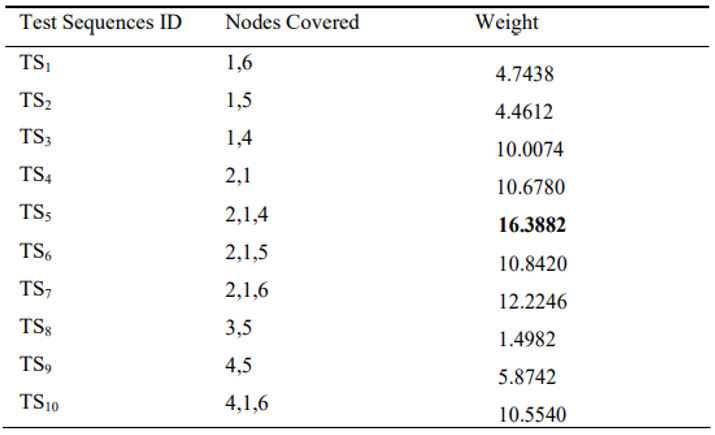
\includegraphics[width=\textwidth,height=\textheight,keepaspectratio]{test_table.PNG}
\end{figure}
 
\par Οι συγγραφείς καταλήγουν ότι «μπορεί εύκολα να διαπιστωθεί ότι σχεδόν το 80\% των σφαλμάτων έχουν καλυφθεί στο 60\% του συνολικού χρόνου. Επομένως, συνάγεται το συμπέρασμα ότι ο αριθμός των σφαλμάτων που αποκαλύπτονται ανά μονάδα χρόνου είναι καλύτερος του της προτεινόμενης μεθοδολογίας».

\par Οι \textcite{kung} από την άλλη χρησιμοποιούν μαθηματικές λύσεις, βασισμένες σε θεωρία γράφων, ώστε να κατασκευάσουν αλγορίθμους που εντοπίζουν σχέσεις εξάρτησης μεταξύ στοιχείων του προγράμματος και άρα ποιοι έλεγχοι πρέπει να μεταβληθούν.

\par Η θεωρία και οι αλγόριθμοι που χρησιμοποιούνται καθώς και οι μέθοδοι αξιοποίησής τους διαφεύγουν της εμβέλειας αυτού του εγγράφου και άρα παραπέμπουμε τον αναγνώστη να διαβάσει την αναφορά ο ίδιος. 
 
\subsection{Αυτοματοποίηση}

Μακράν ο πιο συνηθισμένος και συχνά πιο πρακτικός τρόπος να διευκολύνουμε την επαλήθευση αντικειμενοστραφών προγραμμάτων παραμένει η αυτοματοποίηση των ελέγχων. Αυτή είναι απαραίτητη για τη παράδοση προϊόντος με καλή ποιότητα στον κατάλληλο χρόνο.

\par Η αυτοματοποίηση δοκιμών είναι λογισμικό που αυτοματοποιεί οποιαδήποτε πτυχή της δοκιμής ενός συστήματος εφαρμογών με δυνατότητα παραγωγής δοκιμαστικών εισροών και αναμενόμενων αποτελεσμάτων. Μειώνει τις επαναλαμβανόμενες εργασίες που κάνουμε χειροκίνητα και επίσης μας παρέχει το αποτέλεσμα ως επιτυχία ή αποτυχία.

\par Σύμφωνα με \textcite{claurence}, η κατάλληλη έκταση των αυτοματοποιημένων δοκιμών εξαρτάται από 

\quotebox {
[...] τους στόχους των δοκιμών, τον προϋπολογισμό, τη διαδικασία λογισμικού, το είδος της υπό ανάπτυξη εφαρμογής και τις ιδιαιτερότητες του περιβάλλοντος ανάπτυξης και στόχου. Οι αυτοματοποιημένες δοκιμές εξασφαλίζουν χαμηλό ποσοστό ελαττωμάτων και συνεχή πρόοδο, ενώ οι χειροκίνητες δοκιμές θα οδηγούσαν πολύ γρήγορα σε εξάντληση των ελεγκτών.
}

Προσθέτοντας αργότερα πως:

\quotebox {
Για να συνοψίσουμε τα χαρακτηριστικά των δοκιμών που επιδιώκουμε:

\begin{itemize}
\item Οι δοκιμές \textit{εκτελούν} το σύστημα σε αντίθεση µε τις στατικές αναλύσεις που αναλύουν απλά τον κώδικα.
\item Οι δοκιμές είναι αυτόματες για να αποτρέψουν τα μέλη του έργου να βαρεθούν τις δοκιμές (ή εναλλακτικά για να αποτρέψουν ένα σύστημα που δεν έχει δοκιμαστεί αρκετά).
\item Οι αυτοματοποιημένες δοκιμές δημιουργούν τα δεδομένα δοκιμής, εκτελούν τη δοκιμή και εξετάζουν το αποτέλεσμα αυτόματα.
\item Η επιτυχία ή η αποτυχία της δοκιμής παρατηρείται αυτόματα κατά τη διάρκεια της εκτέλεσης της δοκιμής.
\item Μια σουίτα δοκιμών ορίζει επίσης ένα σύστημα που εκτελείται μαζί με το δοκιμασμένο σύστημα παραγωγής. Ο σκοπός αυτού του εκτεταµένου συστήµατος είναι να εκτελεί τις δοκιµές σε αυτοµατοποιηµένη µορφή.
\item Μια δοκιμή είναι υπόδειγμα. Μια δοκιμή χρησιμοποιεί συγκεκριμένες τιμές για τα δεδομένα εισόδου, τα δεδομένα δοκιμής.
\item Μια δοκιμή είναι επαναλήψιμη και καθορισμένη. Για την ίδια ρύθμιση παράγονται τα ίδια αποτελέσματα.

\end{itemize}
}

\printbibliography

\end{document}
